
\section{IARU-Bandplan für 2 m}
\label{section:iaru_bandplan_2m}
\begin{frame}%STARTCONTENT

\begin{figure}
    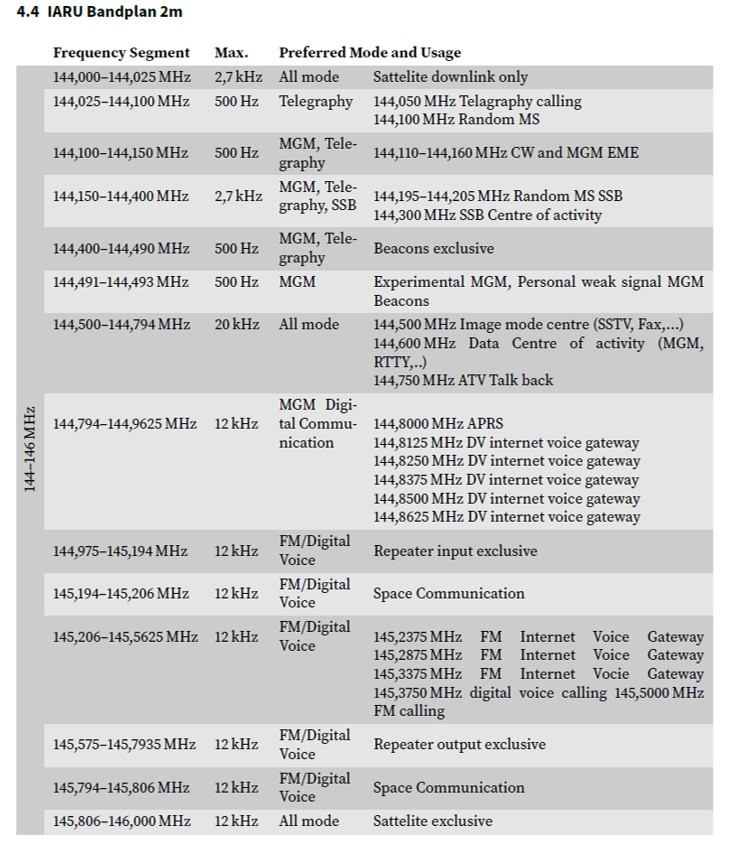
\includegraphics[width=0.85\textwidth]{foto/102}
    \caption{\scriptsize IARU-Bandplan \qty{2}{\metre}}
    \label{n_iaru_bandplan_2m}
\end{figure}

\end{frame}

\begin{frame}
\frametitle{Anruffrequenz}
Um schnell Funkpartner zu finden

\begin{itemize}
  \item FM-Sprechfunk (\enquote{FM calling})
  \item Digitale Telefonie (\enquote{digital voice calling})
  \end{itemize}

\end{frame}

\begin{frame}
\only<1>{
\begin{QQuestion}{BC205}{Welche Frequenz empfiehlt der IARU-Bandplan für einen allgemeinen Anruf mit analoger FM-Telefonie im \qty{2}{m}-Band?}{\qty{145,500}{\MHz}}
{\qty{144,050}{\MHz}}
{\qty{144,800}{\MHz}}
{\qty{145,800}{\MHz}}
\end{QQuestion}

}
\only<2>{
\begin{QQuestion}{BC205}{Welche Frequenz empfiehlt der IARU-Bandplan für einen allgemeinen Anruf mit analoger FM-Telefonie im \qty{2}{m}-Band?}{\textbf{\textcolor{DARCgreen}{\qty{145,500}{\MHz}}}}
{\qty{144,050}{\MHz}}
{\qty{144,800}{\MHz}}
{\qty{145,800}{\MHz}}
\end{QQuestion}

}
\end{frame}

\begin{frame}
\only<1>{
\begin{QQuestion}{BC207}{Welche Frequenz empfiehlt der IARU-Bandplan für einen allgemeinen Anruf mit digitaler Telefonie im \qty{2}{m}-Band?}{\qty{145,500}{\MHz}}
{\qty{145,375}{\MHz}}
{\qty{144,800}{\MHz}}
{\qty{144,195}{\MHz}}
\end{QQuestion}

}
\only<2>{
\begin{QQuestion}{BC207}{Welche Frequenz empfiehlt der IARU-Bandplan für einen allgemeinen Anruf mit digitaler Telefonie im \qty{2}{m}-Band?}{\qty{145,500}{\MHz}}
{\textbf{\textcolor{DARCgreen}{\qty{145,375}{\MHz}}}}
{\qty{144,800}{\MHz}}
{\qty{144,195}{\MHz}}
\end{QQuestion}

}
\end{frame}

\begin{frame}
\frametitle{Frequenzwechsel}
\begin{itemize}
  \item Anruffrequenzen für Anrufe freihalten
  \item Nach Verbindungsaufbau auf eine andere Frequenz verständigen
  \item Nützliche Frequenz aus dem Bandplan entnehmen
  \item Frequenz wechseln
  \end{itemize}
\end{frame}

\begin{frame}
\only<1>{
\begin{QQuestion}{BC209}{Auf welcher der folgenden Frequenzen könnten Sie beispielsweise unter Berücksichtigung des IARU-Bandplans im \qty{2}{\m}-Band eine FM-Telefonieverbindung durchführen?}{\qty{145,450}{\MHz}}
{\qty{144,250}{\MHz}}
{\qty{144,090}{\MHz}}
{\qty{144,450}{\MHz}}
\end{QQuestion}

}
\only<2>{
\begin{QQuestion}{BC209}{Auf welcher der folgenden Frequenzen könnten Sie beispielsweise unter Berücksichtigung des IARU-Bandplans im \qty{2}{\m}-Band eine FM-Telefonieverbindung durchführen?}{\textbf{\textcolor{DARCgreen}{\qty{145,450}{\MHz}}}}
{\qty{144,250}{\MHz}}
{\qty{144,090}{\MHz}}
{\qty{144,450}{\MHz}}
\end{QQuestion}

}
\end{frame}

\begin{frame}
\frametitle{Analoge SSB-Telefonie}
\begin{itemize}
  \item Es gibt keine Anruffrequenz
  \item Stattdessen ein \emph{Aktivitätszentrum} bzw. \emph{center of activity}
  \item Anrufe sollen im Umfeld dieser Frequenz stattfinden
  \item Es kann aber der ganze \enquote{SSB}-Bereich genutzt werden
  \end{itemize}
\end{frame}

\begin{frame}
\only<1>{
\begin{QQuestion}{BC211}{Welche Frequenz bzw. welchen Frequenzbereich sieht der IARU-Bandplan als Aktivitätszentrum für SSB-Telefonie im \qty{2}{m}-Band vor?}{\qty{145,500}{\MHz}}
{\qty{144,300}{\MHz}}
{\qtyrange{144,195}{144,205}{\MHz}}
{\qtyrange{144,110}{144,160}{\MHz}}
\end{QQuestion}

}
\only<2>{
\begin{QQuestion}{BC211}{Welche Frequenz bzw. welchen Frequenzbereich sieht der IARU-Bandplan als Aktivitätszentrum für SSB-Telefonie im \qty{2}{m}-Band vor?}{\qty{145,500}{\MHz}}
{\textbf{\textcolor{DARCgreen}{\qty{144,300}{\MHz}}}}
{\qtyrange{144,195}{144,205}{\MHz}}
{\qtyrange{144,110}{144,160}{\MHz}}
\end{QQuestion}

}
\end{frame}

\begin{frame}
\only<1>{
\begin{QQuestion}{BC210}{Auf welcher der folgenden Frequenzen könnten Sie unter Berücksichtigung des IARU-Bandplans im \qty{2}{m}-Band eine SSB-Telefonieverbindung beispielsweise durchführen?}{\qty{144,800}{\MHz}}
{\qty{145,450}{\MHz}}
{\qty{144,310}{\MHz}}
{\qty{144,450}{\MHz}}
\end{QQuestion}

}
\only<2>{
\begin{QQuestion}{BC210}{Auf welcher der folgenden Frequenzen könnten Sie unter Berücksichtigung des IARU-Bandplans im \qty{2}{m}-Band eine SSB-Telefonieverbindung beispielsweise durchführen?}{\qty{144,800}{\MHz}}
{\qty{145,450}{\MHz}}
{\textbf{\textcolor{DARCgreen}{\qty{144,310}{\MHz}}}}
{\qty{144,450}{\MHz}}
\end{QQuestion}

}
\end{frame}

\begin{frame}
\frametitle{Reservierte Frequenzbereiche}
\begin{itemize}
  \item Satelliten-Up- und Downlink (\enquote{satellite uplink}, \enquote{satellite downlink})
  \item Baken (\enquote{beacons})
  \item Relaisfunkstellen, Eingabe und Ausgabe (\enquote{repeater input}, \enquote{repeater output})
  \item Weltraumkommunikation (\enquote{space communication})
  \item Morsetelegrafie (\enquote{CW})
  \end{itemize}

\end{frame}

\begin{frame}
\only<1>{
\begin{QQuestion}{BC214}{Warum sollten Sie auf \qty{144,125}{\MHz} \underline{keine} Direktverbindung in FM-Telefonie zu einem Funkamateur aufnehmen, der sich im Nachbarort befindet? Der IARU-Bandplan empfiehlt diesen Bereich für die Nutzung durch~...}{Baken.}
{Repeater.}
{Weltraumkommunikation.}
{Morsetelegrafie und schmalbandige digitale Übertragungsverfahren.}
\end{QQuestion}

}
\only<2>{
\begin{QQuestion}{BC214}{Warum sollten Sie auf \qty{144,125}{\MHz} \underline{keine} Direktverbindung in FM-Telefonie zu einem Funkamateur aufnehmen, der sich im Nachbarort befindet? Der IARU-Bandplan empfiehlt diesen Bereich für die Nutzung durch~...}{Baken.}
{Repeater.}
{Weltraumkommunikation.}
{\textbf{\textcolor{DARCgreen}{Morsetelegrafie und schmalbandige digitale Übertragungsverfahren.}}}
\end{QQuestion}

}
\end{frame}

\begin{frame}
\only<1>{
\begin{QQuestion}{BC215}{Warum sollten Sie auf \qty{144,450}{\MHz} \underline{keine} Direktverbindung in FM-Telefonie zu einem Funkamateur aufnehmen, der sich im Nachbarort befindet? Der IARU-Bandplan sieht diesen Bereich exklusiv für die Nutzung durch~...}{Baken vor.}
{Repeater vor.}
{Weltraumkommunikation vor.}
{Morsetelegrafie und schmalbandige digitale Übertragungsverfahren vor.}
\end{QQuestion}

}
\only<2>{
\begin{QQuestion}{BC215}{Warum sollten Sie auf \qty{144,450}{\MHz} \underline{keine} Direktverbindung in FM-Telefonie zu einem Funkamateur aufnehmen, der sich im Nachbarort befindet? Der IARU-Bandplan sieht diesen Bereich exklusiv für die Nutzung durch~...}{\textbf{\textcolor{DARCgreen}{Baken vor.}}}
{Repeater vor.}
{Weltraumkommunikation vor.}
{Morsetelegrafie und schmalbandige digitale Übertragungsverfahren vor.}
\end{QQuestion}

}
\end{frame}

\begin{frame}
\only<1>{
\begin{QQuestion}{BC218}{Warum sollten Sie auf \qty{145,800}{\MHz} \underline{keine} Direktverbindung in FM-Telefonie zu einem Funkamateur aufnehmen, der sich im Nachbarort befindet? Der IARU-Bandplan empfiehlt diesen Bereich für die Nutzung durch ...}{Baken.}
{Repeater.}
{Morsetelegrafie und schmalbandige digitale Übertragungsverfahren.}
{Weltraumkommunikation.}
\end{QQuestion}

}
\only<2>{
\begin{QQuestion}{BC218}{Warum sollten Sie auf \qty{145,800}{\MHz} \underline{keine} Direktverbindung in FM-Telefonie zu einem Funkamateur aufnehmen, der sich im Nachbarort befindet? Der IARU-Bandplan empfiehlt diesen Bereich für die Nutzung durch ...}{Baken.}
{Repeater.}
{Morsetelegrafie und schmalbandige digitale Übertragungsverfahren.}
{\textbf{\textcolor{DARCgreen}{Weltraumkommunikation.}}}
\end{QQuestion}

}
\end{frame}

\begin{frame}
\only<1>{
\begin{QQuestion}{BC217}{Warum sollten Sie auf \qty{145,600}{\MHz} \underline{keine} Direktverbindung in FM-Telefonie zu einem Funkamateur aufnehmen, der sich im Nachbarort befindet? Der IARU-Bandplan empfiehlt diesen Bereich für die Nutzung durch ...}{Weltraumkommunikation.}
{Repeater.}
{Morsetelegrafie und schmalbandige digitale Übertragungsverfahren.}
{Baken.}
\end{QQuestion}

}
\only<2>{
\begin{QQuestion}{BC217}{Warum sollten Sie auf \qty{145,600}{\MHz} \underline{keine} Direktverbindung in FM-Telefonie zu einem Funkamateur aufnehmen, der sich im Nachbarort befindet? Der IARU-Bandplan empfiehlt diesen Bereich für die Nutzung durch ...}{Weltraumkommunikation.}
{\textbf{\textcolor{DARCgreen}{Repeater.}}}
{Morsetelegrafie und schmalbandige digitale Übertragungsverfahren.}
{Baken.}
\end{QQuestion}

}
\end{frame}

\begin{frame}
\only<1>{
\begin{QQuestion}{BC213}{Warum sollten Sie RTTY, PSK31 oder FT8 \underline{nicht} auf \qty{144,075}{MHz}  verwenden? Der IARU-Bandplan empfiehlt~...}{diesen Bereich bevorzugt für Morsetelegrafie zu nutzen.}
{in diesem Bereich maximal \qty{500}{\Hz} Bandbreite zu belegen, damit der Bereich besser genutzt werden kann.}
{den Einsatz von Computern für die Signalerzeugung zu vermeiden.}
{digitale Verfahren oberhalb von \qty{430}{\MHz} durchzuführen, da dort mehr Bandbreite zur Verfügung steht.}
\end{QQuestion}

}
\only<2>{
\begin{QQuestion}{BC213}{Warum sollten Sie RTTY, PSK31 oder FT8 \underline{nicht} auf \qty{144,075}{MHz}  verwenden? Der IARU-Bandplan empfiehlt~...}{\textbf{\textcolor{DARCgreen}{diesen Bereich bevorzugt für Morsetelegrafie zu nutzen.}}}
{in diesem Bereich maximal \qty{500}{\Hz} Bandbreite zu belegen, damit der Bereich besser genutzt werden kann.}
{den Einsatz von Computern für die Signalerzeugung zu vermeiden.}
{digitale Verfahren oberhalb von \qty{430}{\MHz} durchzuführen, da dort mehr Bandbreite zur Verfügung steht.}
\end{QQuestion}

}
\end{frame}%ENDCONTENT
